\documentclass[a4paper,12pt]{report}
\usepackage[utf8]{inputenc}
\usepackage[T1]{fontenc}
\usepackage[english]{babel}
\usepackage{lmodern}

%Figure progressive enumeration
\usepackage{chngcntr}
\counterwithin{figure}{chapter}
\counterwithin{table}{chapter}

%package used to enumerate figures
\usepackage[labelfont=bf]{caption}

%hyperref for interactive PDF index
\usepackage[bookmarks, colorlinks, breaklinks]{hyperref}
\hypersetup{linkcolor=black, citecolor=black, filecolor=black, urlcolor=black}

%Package required to use special symbols
\usepackage{amsmath, amssymb}

%Package required to use figures
\usepackage{graphicx}
\usepackage{subfig}

%Include the bibliography in the table of contents
\usepackage{tocbibind}

%Package used to insert figures at the specified position
\usepackage{float}
\usepackage{longtable}

%Our chapters must be called sections
\addto\captionsenglish{\renewcommand{\chaptername}{Section}}

\begin{document}

	%Code for title page
	\begin{titlepage}
		\centering
		
\includegraphics[width=0.20\textwidth]{./pictures/logo_polimi.png}\par

		{Politecnico di Milano \\ AA 2018-2019} \par
		\vspace{1.5cm}

		{Computer Science and Engineering}\par
		\Large{Software Engineering II}\par
		\vspace{1.0cm}

		
\includegraphics[width=1.00\textwidth]{./pictures/logo_trackme.png}\par
		{\LARGE \textbf{Requirements Analysis and Specification Document} \par}
		\vspace{1.0cm}
		{\Large Stefano Bagarin\\ Alessandra Pasini\par}
		\vspace{2cm}
		\vfill

		% Bottom of the page
		{\large Document version: 1.0\par}
		{\large \today \par}
	\end{titlepage}

	%Make the table of contents
	\tableofcontents

	%INTRODUCTION
	\chapter{Introduction}
	\label{ch:Introduction}

	\section{Purpose}
	The goal of the Design Document (DD) is to provide to the software development team in charge of the making of the project an overall description of the architecture it will need to have and some tecnical aspects. This is needed to help to coordinate each member of the team and make them work with an unified vision of the software. \\
To reach the presented goal, in this document are described the design of the architecture with some UML diagrams, the design of the user interfaces already described in the RASD document, the requirements traceability and the plan made for implementing, integrating and testing the software.


	\section{Scope}
	\subsection{Description of the given problem}

As already said in the previous section \textit{TrackMe}'s system as the aim to provide different applications to the different actors.
\begin{itemize}
	\item {\textit{D4H and ASOS} app is designed to provide the users with an overview of their health parameters by obtaining them from the device associated to the smartphone that runs it. The device should be able to collect health parameters such as the heart beat and send them to the main app running on the smartphone. If the user has activated the \textit{ASOS} service everytime that a new value is collected the app checks if it is higher or not than the trashold value:
		\begin{itemize}
			\item {if it is upper it is stored in the database;}
			\item {if it is lower the \textit{ASOS} service will be activated and it will contact the outside SOS service in less than 5 seconds from the time the parameters started to be below the threshold. By contacting the SOS service \textit{ASOS} will also give the location of the user who needs medical help.}
		\end{itemize}
		The user can always choose to activate the \textit{ASOS} service by subscribing to it in the designated area. The user can also monitor his/her health parameters by looking the specific app's area.\\
		Anytime a third party will ask to accede to the single user's data the app will send a notification to the specific user to get permission to share his/her data. The user can accept or deny the request.}

	\item{\textit{D4H} app is designed to provide the third parties with the possibility to require single user's or group of users' data.
		If the third party wants to accede to the data of  a specific user it must have his/her secure number or fiscal code. The app is than in charge to ask to the specific user if he/she wants to share his/her data with the third party: if the user accepts, data will be shared; if he/she denies, the third party will receive a notification saying that.\\
		To obtain data of groups of users the third parties must specify some contraints to define the type of data and the type of uses they are interested in; this means that the query can be personalized depending on which type of data the third parties need. The app accepts those requests and sends data if and only if the quantity of users that respect the query's parameters is heigher than 1000; this threshold has been imposed to guarantee users' privacy. in case the number of users is lower than 1000 the third party will receive a notification saying that.\\
		Throught this app a third party can also subscribe for new data, once a request has been accepted the app asks if it would like to receive more data related to the single user or to the group of users of the request.}
		
\end{itemize}

\subsection{World and Machine}
The aim of this subsection is to describe the problem following the World and Machine model. The World domain is the set of all real-life events in which the Machine will be introduced and in which its actions will be observed. The Machine domain is the set of all phenomena which it can control such as algorithms, devices, inputs from the world.\\
Those two domains are connected via Shared Phenomena which are World's events and Machine's actions which are observable by both domains.

\begin{figure}[h!]
	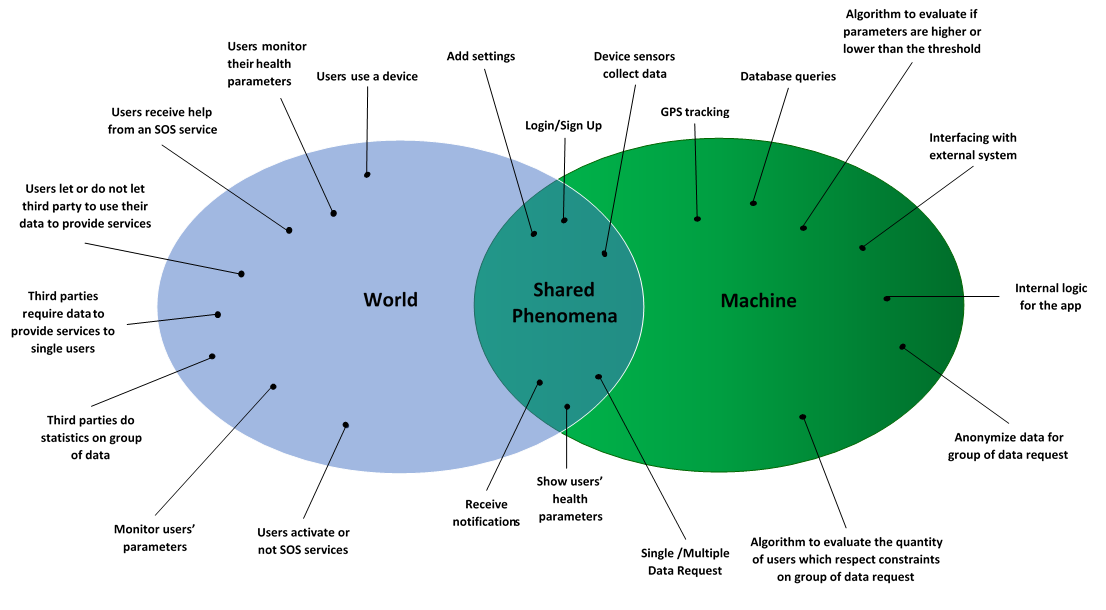
\includegraphics[width=1.00\textwidth]{./pictures/world_machine.png}\par
	\caption{Figure 1: World and Machine diagram}
\end{figure}

	\section{Goals}
	{The goals of \hbox{\emph{TrackMe}} are the following:
\vspace{0.3cm}

\begin{itemize}
	\item[${\textbf{[G1]}}$] {Allows a person to register and to have a personal area to which he/she can access with his credentials.}
	\item[${\textbf{[G2]}}$] {Allows the third party to register and to have a personal area to which it can access with his credentials.}
	\item[${\textbf{[G3]}}$] {Allows the third party to require data.
				\begin{itemize}
					\item[${\textbf{[G3.1]}}$] {Third party can require single person's data.}
					\item[${\textbf{[G3.2]}}$] {Third party can require anonymized data of group of people.}
				\end{itemize}}
	\item[${\textbf{[G4]}}$] {Allows the user to accept or not to let a third party to have access to his/her data.}
	\item[${\textbf{[G5]}}$] {Allows third party to subscribe for new data.}
	\item[${\textbf{[G6]}}$] {Allows third party to obtain the required data if the request has been accepted, a notification if it has been refused.}
	\item[${\textbf{[G7]}}$] {Allows users to activate or deactivate the \hbox{\emph{ASOS}} service on top of \hbox{\emph{D4H}}.}
	\item[${\textbf{[G8]}}$] {Allows an unhealty user to receive quick help if have the \hbox{\emph{ASOS}} service activated on his account.}

	
\end{itemize}


	\section{Definitions, Acronyms and Abbreviations}
	\subsection{Definitions}

\subsection{Acronyms}
	
\subsection{Abbreviations }
	\begin{itemize}
		\item {[Gn]: n-th goal}
		\item {[Dn]: n-th domain assumption}
		\item {[Rn]: n-th requiremnt}
	\end{itemize}




	\section{References}

	\section{Document Structure}

	%Overall Description
	\chapter{Overall Description}
	\label{ch:Overall_Description}

	\section{Product Perspective}
	The main goals of the \hbox{\emph{Track Me}}'s system are to provide to the third parties a big pool of users from which can gather data (offered by the base service of \hbox{\emph{D4H}}) and to provide to the users a timely medical  assistance in case of illness (offered by the SOS service on top of \hbox{\emph{D4H}}). The system is designed to be used as two different application: one for users and one for third parties. The users' application sends data about them to \hbox{\emph{Track Me}}'s servers where then they can be collected by third parties throught theirs application by making a request for receiving data of a specific users or anonimized data of multiple users. \hbox{\emph{Track Me}} uses user's data also for garanting a timely medical assistance to the users who have activated the \hbox{\emph{ASOS}} service in case of drop of theirs health parameters gathered by theirs application by contacting an external SOS service.\\

The following diagram is provided to better describe the \hbox{\emph{Track Me}}'s system:
\begin{figure}
	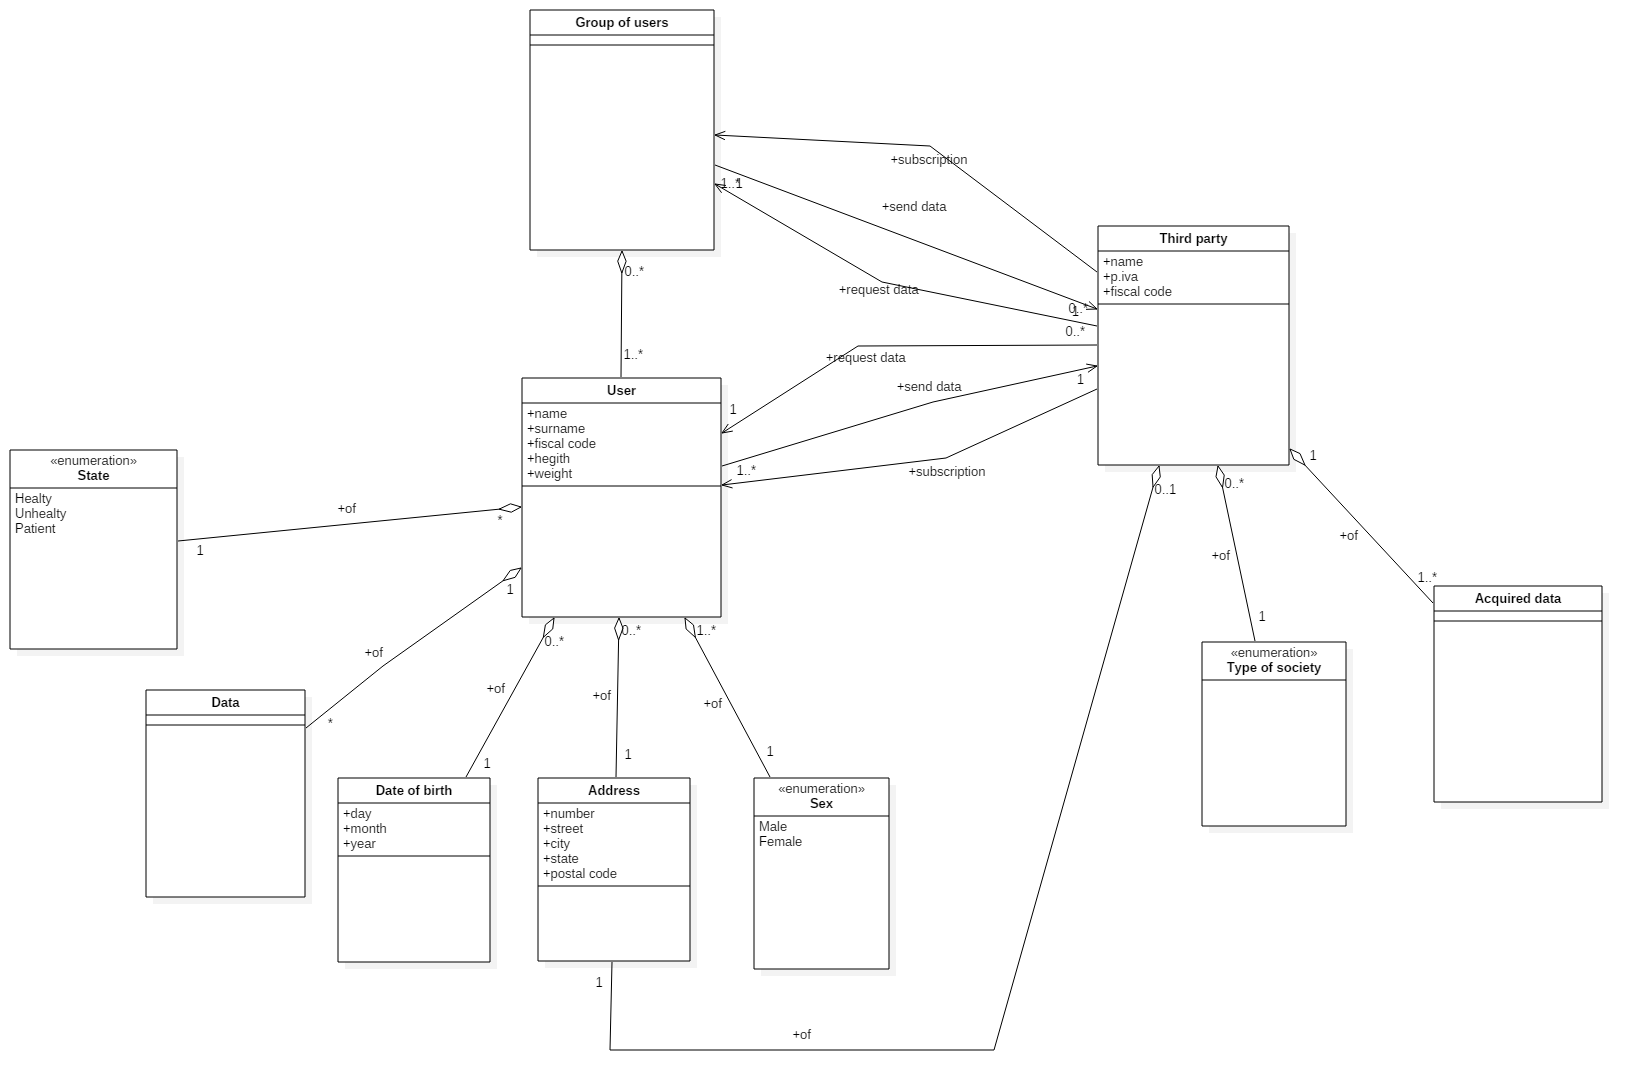
\includegraphics[width=1.00\textwidth]{./pictures/uml_v1.png}\par
	\caption{Figure 1: Class Diagram}
\end{figure}
\FloatBarrier
\vspace{0.3cm}As shown, all the system is centered on garanting data to third parties of users or groups of users and garanting medical assistance for the users who have activated the SOS service (the attribute "state" of the user is intended right for this scope).

\vspace{0.5cm}In the next diagrams the processes of acquisition data of users and groups of users by third parties are analyzed:
\begin{figure}[!h]
	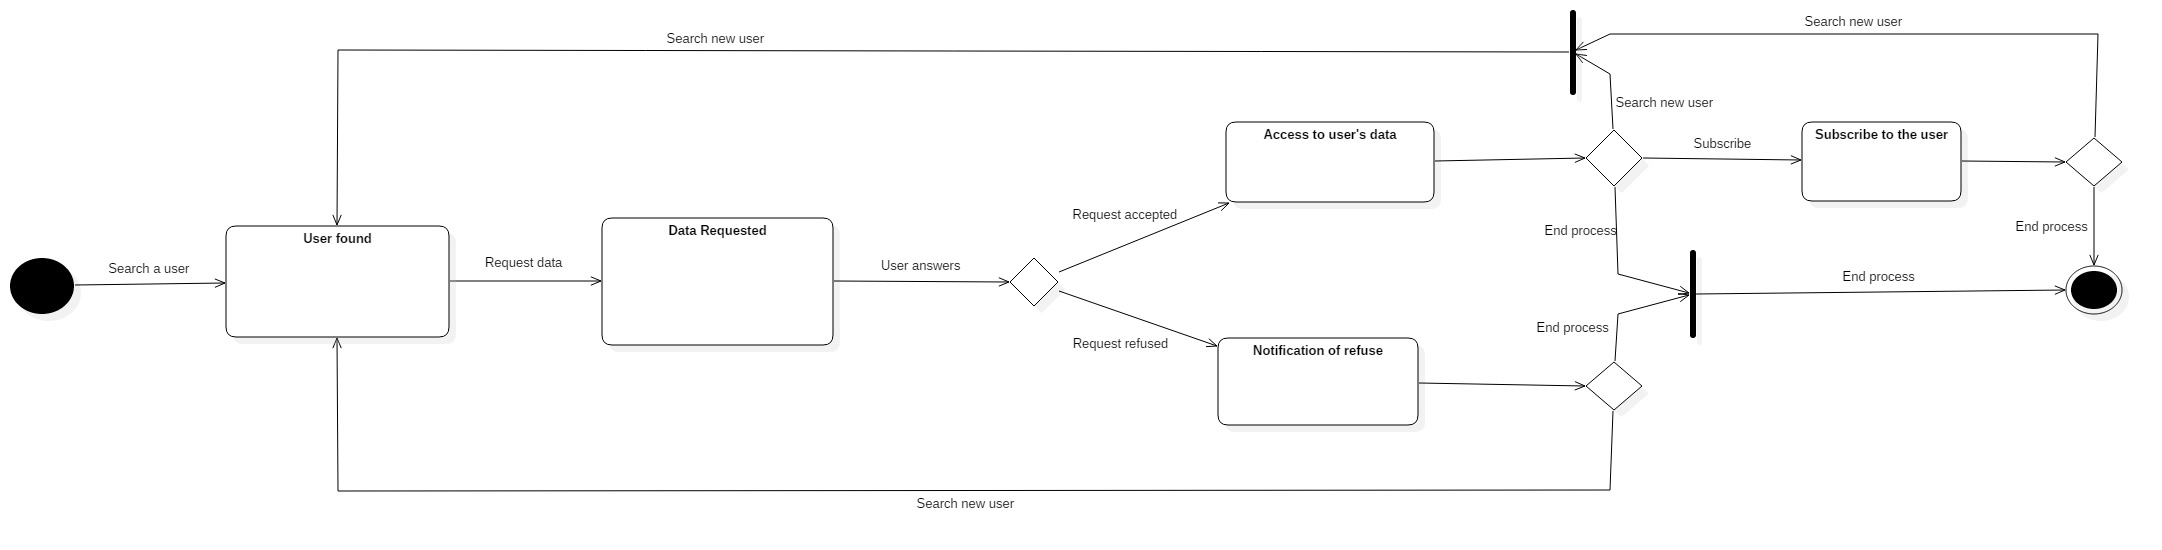
\includegraphics[width=1.00\textwidth]{./pictures/State_diagram_users_v_1.jpg}\par
	\caption{Figure 2: State diagram of the process of acquisition data of users by third parties.}
\end{figure}
\FloatBarrier
\vspace{0.3cm}

\begin{figure}[!h]
	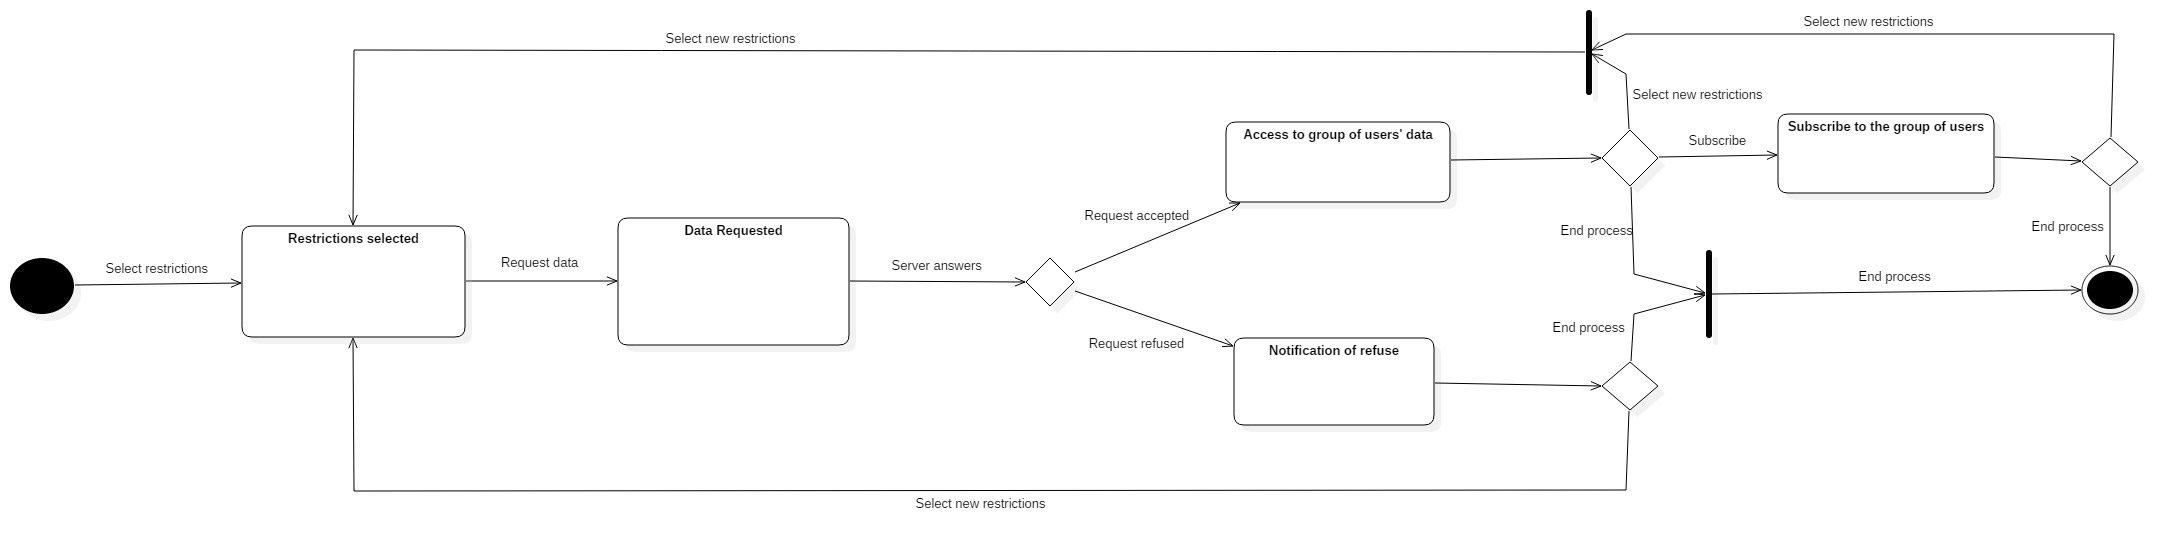
\includegraphics[width=1.00\textwidth]{./pictures/State_diagram_groups_v_1.jpg}\par
	\caption{Figure 3: State diagram of the process of acquisition data of groups of users by third parties.} 
\end{figure}
\FloatBarrier
\vspace{0.3cm}Notice that both diagrams describe the sequence of actions to make a single or multiple requests and relavite subscriptions to users/groups of users. Notice also that the two diagrams have a similar structure but are conceptually different and takes different actors (in particular no user takes an action in the second diagram).

	\section{Product Functions}

	\section{User Characteristics}
	The following actors are the users of those two applications:

\begin{itemize}
	\item{\textbf{User:}\\ a person that is successfully registrated to \textit{D4H} and \textit{ASOS} and that is able to use all its 				services to monitor his/her health parameters.}

	\item{\textbf{Third Party:}\\ a company, a foundation or any other ype of institution that is succesfully registered to \textit{D4H} 		and that is able to use all its services to obtain data.}
\end{itemize}

	\section{Assumptions and Dependencies}
	{The domain assumptions of \hbox{\emph{D4H}} are the following:
\vspace{0.3cm}

\begin{itemize}
	\item[$\textbf{[D1]}$] {The user has a device linked to his smartphone.}
	\item[$\textbf{[D2]}$] {The user's smartphone can provide an accurate enough current location.}
	\item[$\textbf{[D3]}$] {The user's device can provide accurate enough healt parameters.}
	\item[$\textbf{[D4]}$] {The user's smartphone can provide constantly data  to \hbox{\emph{D4H}}.}
	\item[$\textbf{[D5]}$] {There is an SOS service that has the capability to receive emergency calls by ASOS.
	\begin{itemize}
		\item[$\textbf{[D5.1]}$] {The SOS service has the capability to receive data about the unhealty user.}
		\item[$\textbf{[D5.2]}$] {The SOS service has the capability to send assistance to the unhealty user.}
	\end{itemize}}
	
\end{itemize}


	%Specific Requirements
	\chapter{Specific Requirements}
	\label{ch:Specific_Requirements}

	\section{External Interface Requirements}
	\subsection{User Interface}

The following mockups represent a basic idea of how the users' mobile app will look like in the first 
release. 

\begin{figure}[h!]
	\centering
 	 \begin{minipage}[b]{0.25\textwidth}
    		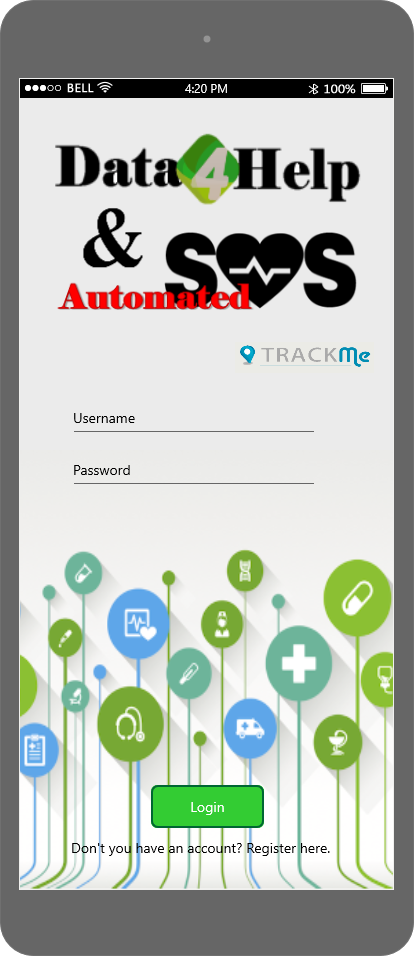
\includegraphics[width=\textwidth]{./pictures/login_user.png}
    		\caption{Mock up - Login screen.}
  	\end{minipage}
	\hfill
 	\begin{minipage}[b]{0.25\textwidth}
    		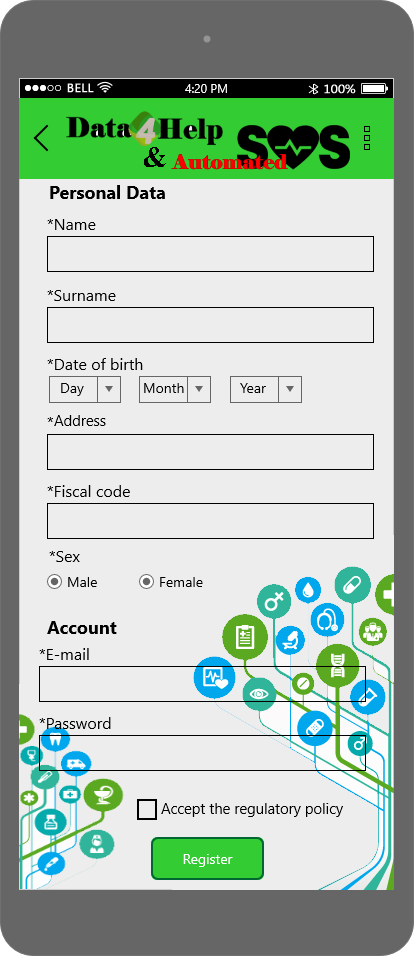
\includegraphics[width=\textwidth]{./pictures/user_registration.png}
    		\caption{Mock up - Registration.}
	\end{minipage}
	\hfill
	\begin{minipage}[b]{0.25\textwidth}
    		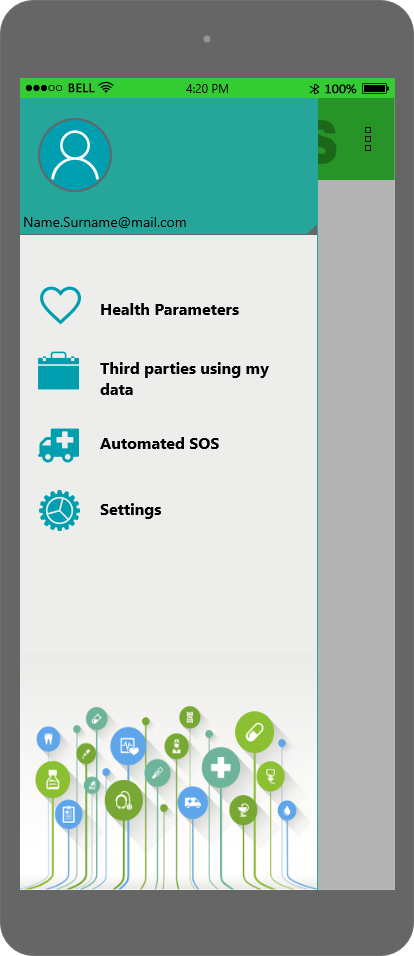
\includegraphics[width=\textwidth]{./pictures/menu.png}
    		\caption{Mock up - Menu.}
	\end{minipage}
\end{figure}

\begin{figure}[h!]
	\centering
 	\begin{minipage}[b]{0.25\textwidth}
    		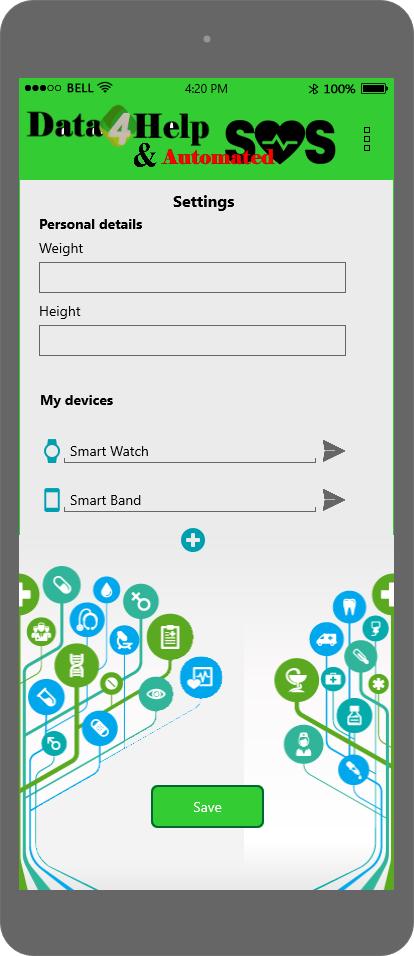
\includegraphics[width=\textwidth]{./pictures/settings.png}
    		\caption{Mock up - Settings.\\}
	\end{minipage}
	\hfill
	\begin{minipage}[b]{0.25\textwidth}
    		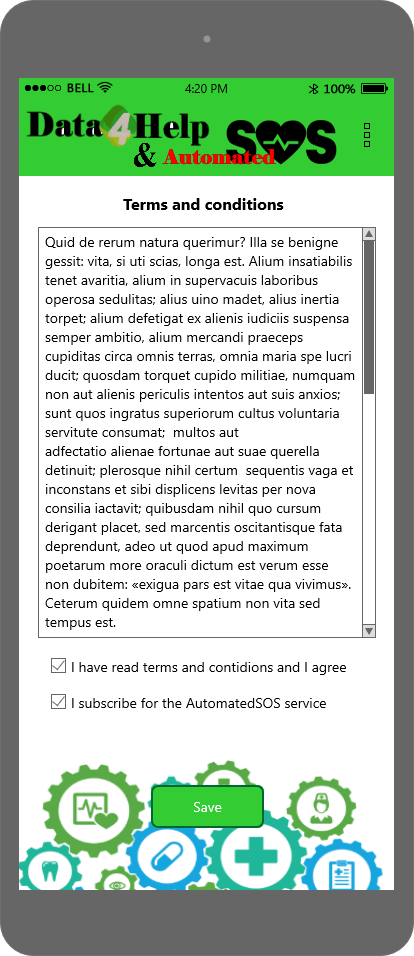
\includegraphics[width=\textwidth]{./pictures/terms_and_conditions.png}
    		\caption{Mock up - Subscribe to \textit{ASOS}.}
	\end{minipage}
	\hfill
	\begin{minipage}[b]{0.25\textwidth}
    		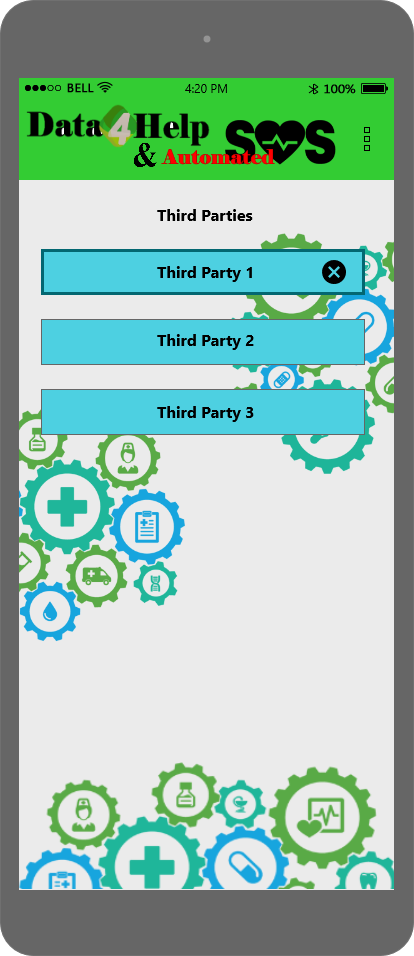
\includegraphics[width=\textwidth]{./pictures/third_party_page.png}
    		\caption{Mock up - Third party using my data.}
	\end{minipage}
\end{figure}

\begin{figure}[h!]
	\centering
 	\begin{minipage}[b]{0.25\textwidth}
    		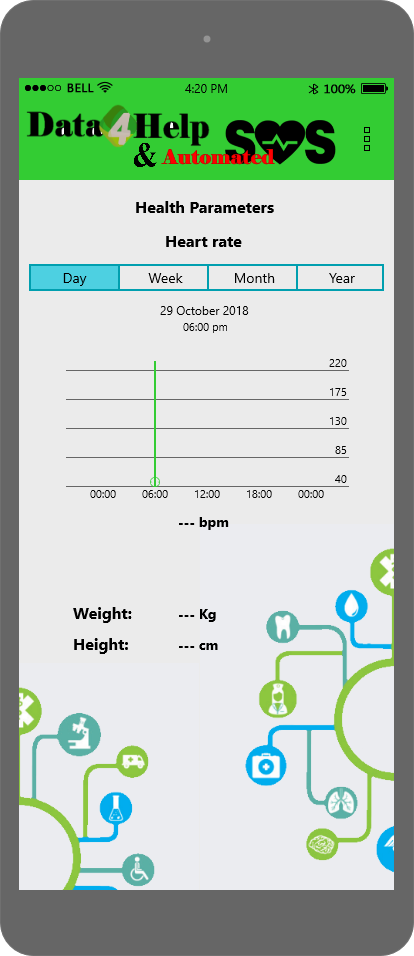
\includegraphics[width=\textwidth]{./pictures/health_param.png}
    		\caption{Mock up - Health parameter.}
	\end{minipage}
	\hfill
	\begin{minipage}[b]{0.25\textwidth}
    		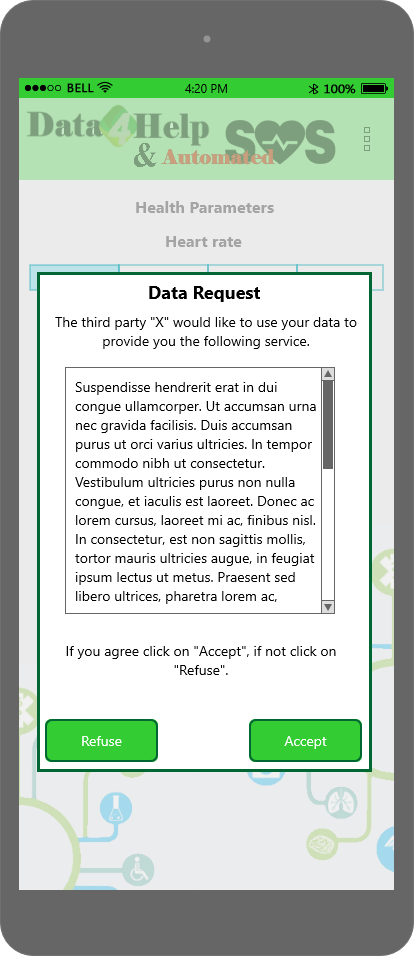
\includegraphics[width=\textwidth]{./pictures/notification.png}
    		\caption{Mock up - Allert to accept or deny .}
	\end{minipage}
\end{figure}



\subsection{Thrid Party Interface}

The following mockups represent a basic idea of how the third party's mobile app will look like in the first 
release. 

\begin{figure}[h!]
	\centering
 	 \begin{minipage}[b]{0.25\textwidth}
    		
\includegraphics[width=\textwidth]{./pictures/login_3p.png}
    		\caption{Mock up - Login screen.\\}
  	\end{minipage}
	\hfill
 	\begin{minipage}[b]{0.25\textwidth}
    		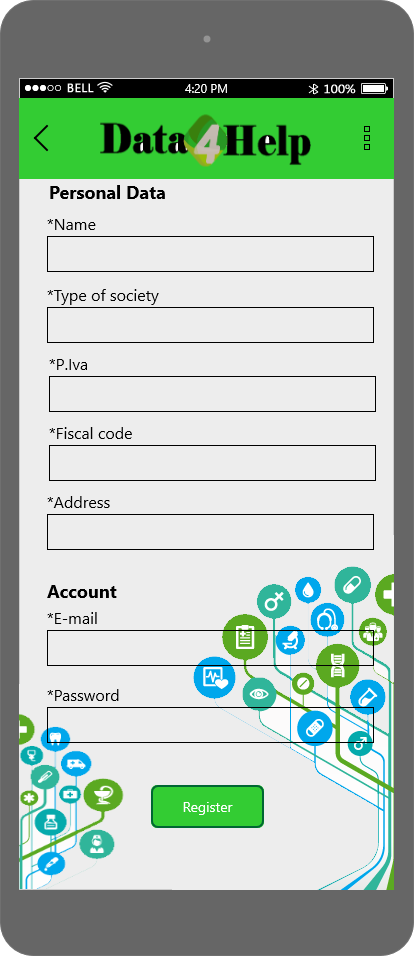
\includegraphics[width=\textwidth]{./pictures/3p_registration.png}
    		\caption{Mock up - Registration.}
	\end{minipage}
	\hfill
 	\begin{minipage}[b]{0.25\textwidth}
    		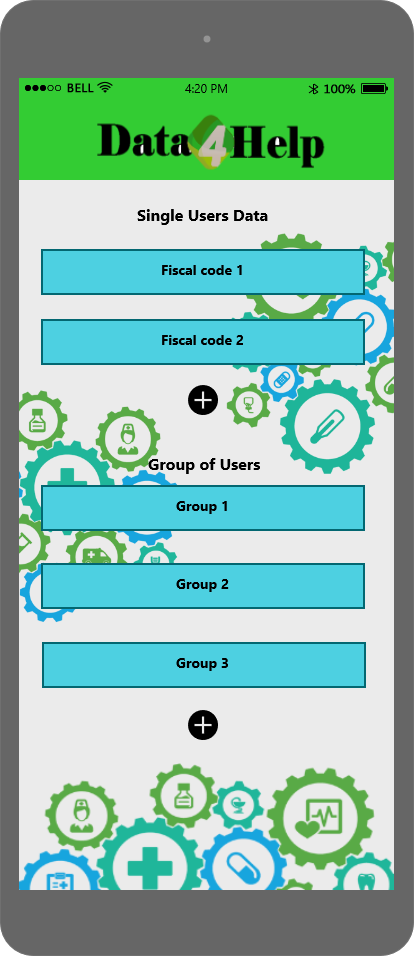
\includegraphics[width=\textwidth]{./pictures/main_scene.png}
    		\caption{Mock up - Main scene.}
	\end{minipage}
\end{figure}
 
\vspace{7cm}
   
\begin{figure}[h!]
	\centering
 	 \begin{minipage}[b]{0.25\textwidth}
    		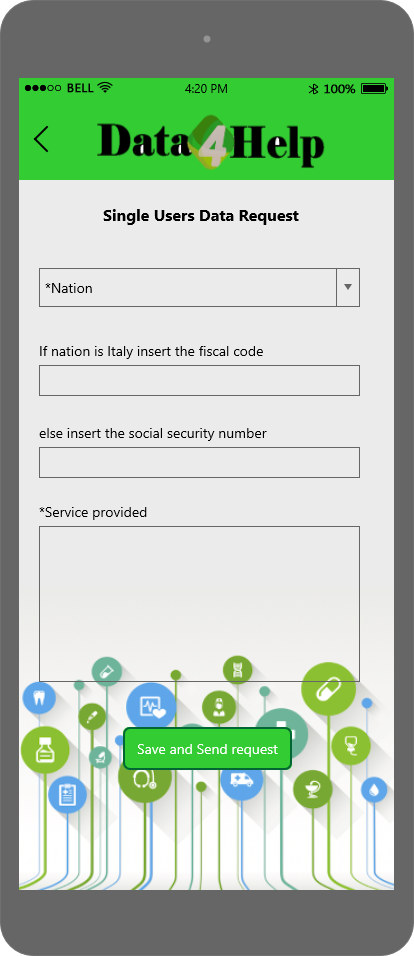
\includegraphics[width=\textwidth]{./pictures/single_user_request.png}
    		\caption{Mock up - Single data request.}
  	\end{minipage}
	\hfill
 	\begin{minipage}[b]{0.25\textwidth}
    		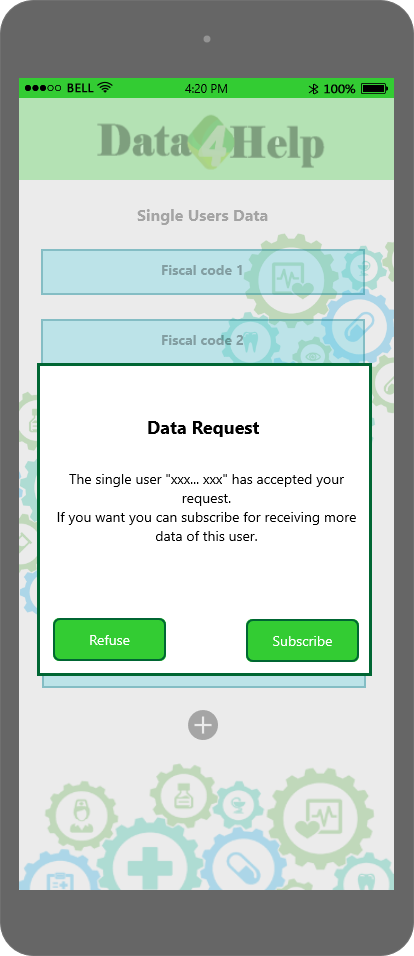
\includegraphics[width=\textwidth]{./pictures/single_user_accept.png}
    		\caption{Mock up - Positive notification.}
	\end{minipage}
	\hfill
 	\begin{minipage}[b]{0.25\textwidth}
    		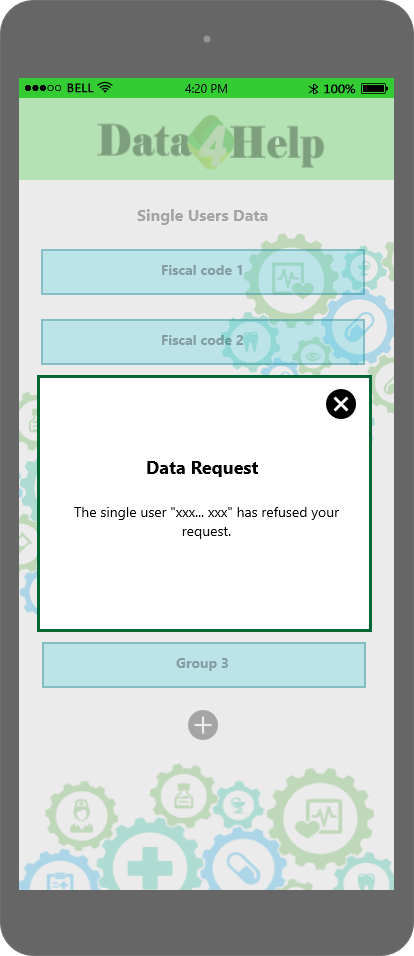
\includegraphics[width=\textwidth]{./pictures/single_user_refuse.png}
    		\caption{Mock up - Negative notification.}
	\end{minipage}
\end{figure}

\begin{figure}[h!]
	\centering
 	\begin{minipage}[b]{0.25\textwidth}
    		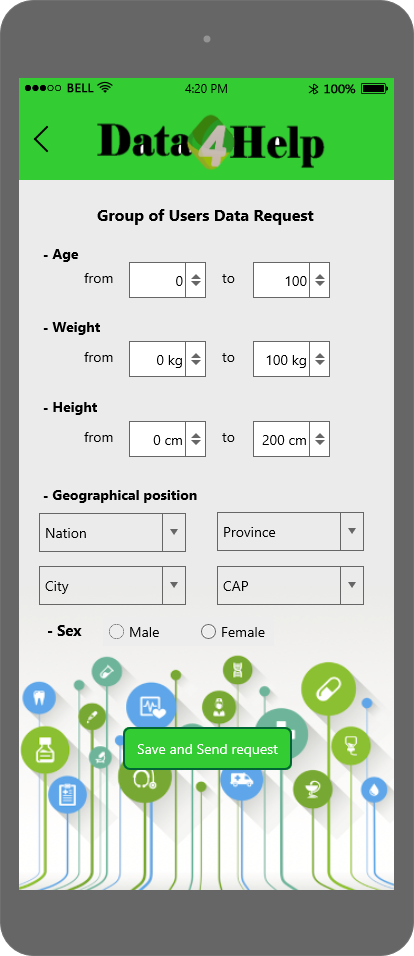
\includegraphics[width=\textwidth]{./pictures/group_request.png}
    		\caption{Mock up - Group of data request.}
	\end{minipage}
	\hfill
	\begin{minipage}[b]{0.25\textwidth}
    		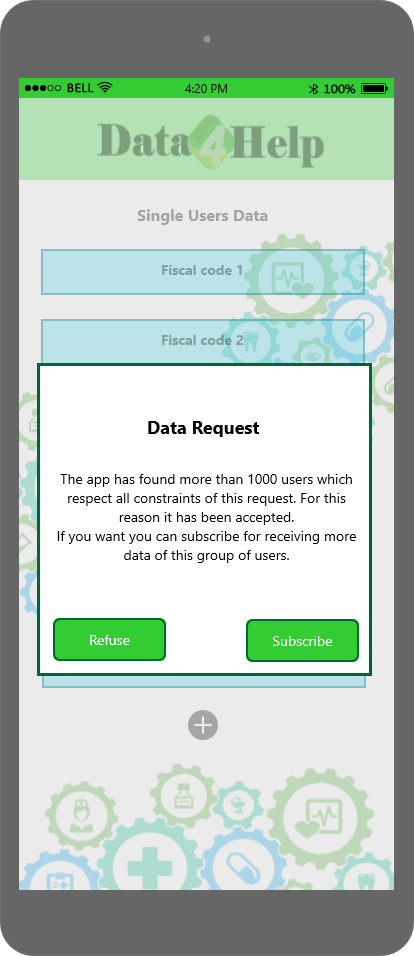
\includegraphics[width=\textwidth]{./pictures/group_accept.png}
    		\caption{Mock up - Positive notification.}
	\end{minipage}
	\hfill
	\begin{minipage}[b]{0.25\textwidth}
    		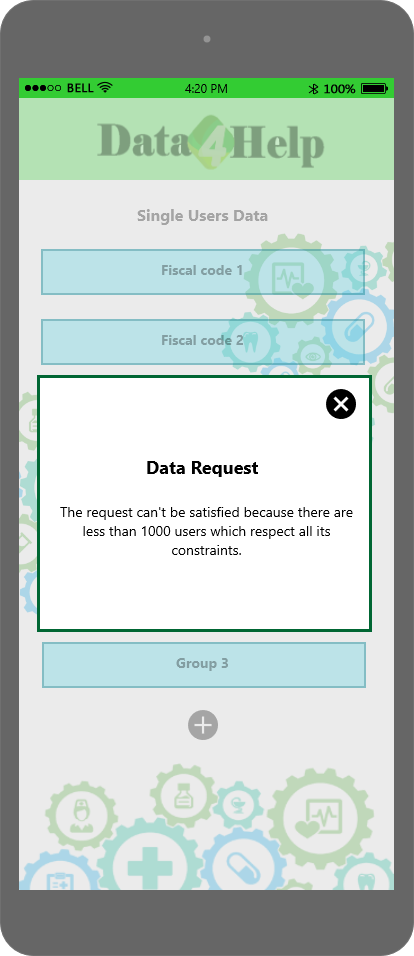
\includegraphics[width=\textwidth]{./pictures/group_refuse.png}
    		\caption{Mock up - Negative notification.}
	\end{minipage}
\end{figure}

\begin{figure}[h!]
	\centering
 	\begin{minipage}[b]{0.25\textwidth}
    		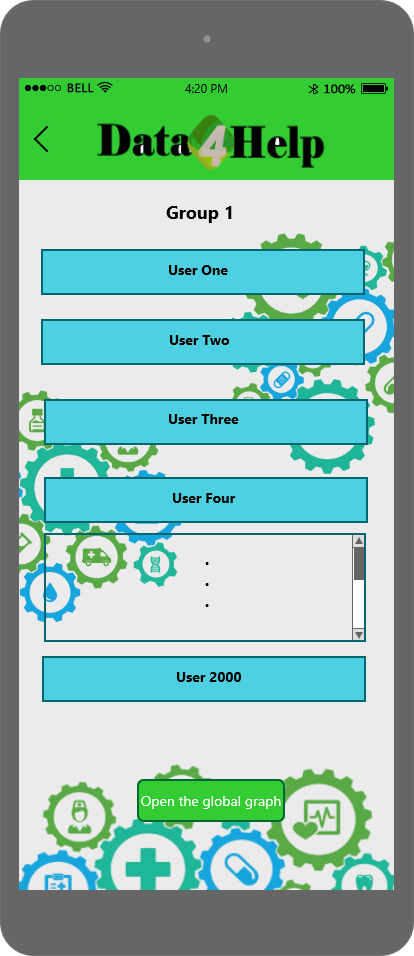
\includegraphics[width=\textwidth]{./pictures/group1.png}
    		\caption{Mock up - Users in a group.}
	\end{minipage}
	\hfill
	\begin{minipage}[b]{0.25\textwidth}
    		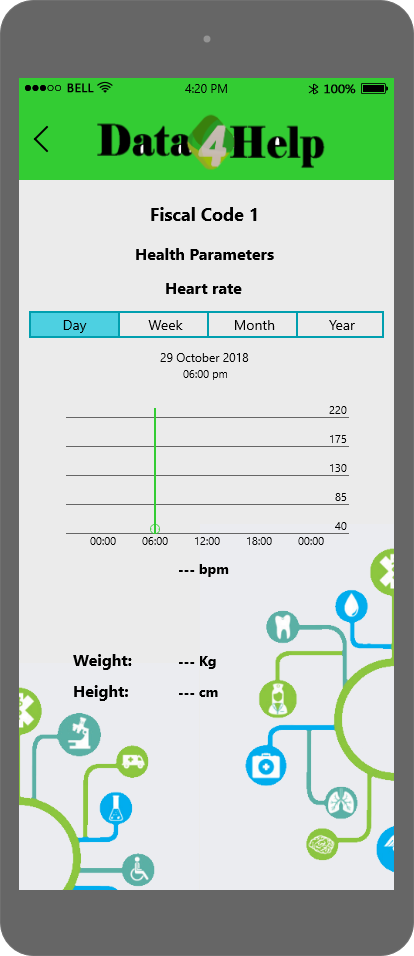
\includegraphics[width=\textwidth]{./pictures/user1.png}
    		\caption{Mock up - Single user's parameter.}
	\end{minipage}
	\hfill
	\begin{minipage}[b]{0.25\textwidth}
    		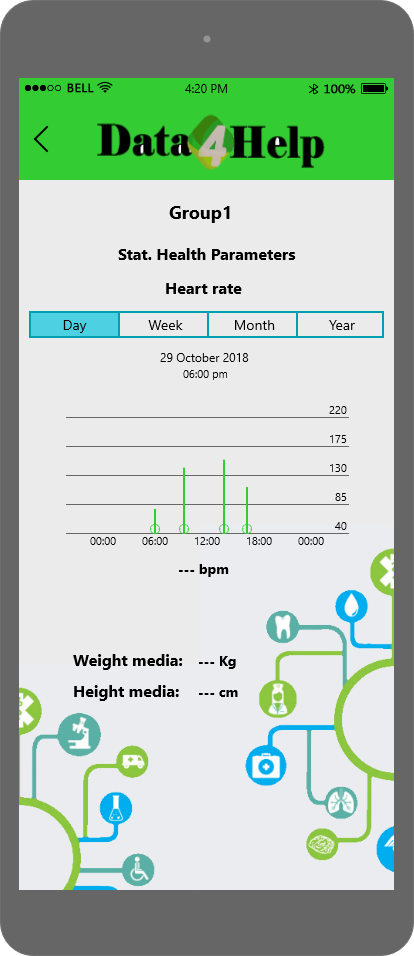
\includegraphics[width=\textwidth]{./pictures/group_stat.png}
    		\caption{Mock up - Statistic par. of a group.}
	\end{minipage}
\end{figure}

	\section{Scenarios}
	\subsection{Scenario 1}
Matteo bought a new smart watch which is compatible with his smartphone and, because of this, he would like to download on his phone an application to monitor his health parameters. 
A friend of him recommended the \textit{D4H} and \textit{ASOS} app and Matteo immediately downloaded it. After he registered himself by giving some personal data, his e-mail and by choosing a password he added some information in settings:
\begin{itemize}
	\item {Matteo inserted his weight and height;}
	\item {he linked his smart watch to the smarphone throught the application to obtain the health parameter;}
\end{itemize}
Then he accepted to activate the \textit{ASOS} service by going in the \textit{ASOS} are in the main menu.
Matteo started to use this application and now he can constantly check his health parameters and see all third parties which has required and which use his data.

\subsection{Scenario 2}
The Health-Tech society would like to obtain data of group of users to analyze and to do some inference on them without spend money to develop a software to collect data from users.This society decides to download the \textit{D4H} application.
After the registration done by giving some personal data, e-mail and a chosen password Health-Text logins to his personal area and can start to require data of a group of users. To require those data the society puts some constraint to obtain data of a specific group of users:
\begin{itemize}
	\item {users must have an age between 20 and 30;}
	\item {users can be both male or female;}
	\item {the society wants to analyze data of users with a weight between 50 kg and 70 kg;}
	\item {users must have a height between 160 cm and 180 cm;}
	\item {they must live in Lombardy;}
\end{itemize}
After a while the app notifies that the request has been accepted because the number of users that respect the constraints is higher than the treshold applied to guarantee the users' privacy.
%The society also subscribes to receive other data of this group of users.

\subsection{Scenario 3}
The Health-Tech society would like to obtain data of a group of users to analyze them. It specifies those constraints for the group of users:
\begin{itemize}
	\item {users must have an age between 16 and 18;}
	\item {users must be male;}
	\item {the society wants to analyze data of users with a weight grater than 100 kg;}
	\item {users must have a height between 160 cm and 180 cm;}
	\item {they must live in Sondrio;}
\end{itemize}
After a while the app notifies that the request has been denied because the number of users which respect the constraints is smaller than the treshold applied to guarantee the users' privacy. 

\subsection{Scenario 4}
The Health-Tech society would like to provide some personalized services to a user. An employee enters in the society's  \textit{D4H} personal area and does a request for obtaining the specific user's data. 
To do it Health-Tech must have a NumberId related to the user or it must have his/her fiscal code and it must explain the reason why it is requiring those data. After a while the app notify that the user has accepted the request and so the society starts to receive data and subscribes for obtaining new data from the user.\\
The app constantly sends the user's data to the Health-Tech personal area.

\subsection{Scenario 5}
The Health-Tech society would like to provide some personalized services to a user. An employee enters in the society's  \textit{D4H} personal area and does a request for obtaining the specific user's data. 
To do it Health-Tech must have a NumberId related to the user or it must have his/her fiscal code and it must explain the reason why it is requiring those data. After a while the app notify that the user didn't accept the request; the request is delated and the employee close the app.

\subsection{Scenario 6}
Diana is at university when the \textit{D4H} and \textit{ASOS} app sends her a notification requiring to accept or deny the possibility to share her data to a third party.
She has chosen to deny it because she was not interested in the proposed service.

\subsection{Scenario 7}
Edoardo is at work when the \textit{D4H} and \textit{ASOS} app sends him a notification requiring to accept or deny the possibility to shere his data to a third party.
He has chosen to accept it bacause he is interested in the proposed service. As soon as he has accepted he goes in the menu and enters in the area which shows all third parties. He can see that the new one has been added immediately.

\subsection{Scenario 8}
Rosaria is walking around the street, she is going to take a coffee with her niece when she has an heart attack. Fortunately she is dressing up her smart watch which takes over that her health parameters are lower than the threshold. The app contacts the SOS service and sends to it Rosaria's personal details and data and her location in less than 5 seconds from the detaction. The SOS service immediately sends her an ambulance which brings her to the hospital in time to save her.


	\section{Functional Requirements} 
	\vspace{0.3cm}

\begin{itemize}

	\item[${\textbf{[G1]}}$] {\textbf{Allows a person to register and to have a personal area to which he/she can access with his credentials.}
		\begin{itemize}
			\item[$\textbf{[R1]}$] {A person can register in the application by providing his personal data, a unique e-mail and a password.}
			\item[$\textbf{[D1]}$] {The user has a device linked to his smartphone.}
			\item[$\textbf{[R2]}$] {A user can log in by providing his e-mail and password.}
			\item[$\textbf{[R3]}$] {Each user has a personal area associated with his credentials.
				\begin{itemize}
					\item[$\textbf{[R3.1]}$] {A user can see the third parties subscribed to his data in his personal area.}
					\item[$\textbf{[R3.2]}$] {A user can add weight and height in his personal area.}
					\item[$\textbf{[R3.3]}$] {A user can link his device to the app in his personal area.}
				\end{itemize}}
		\end{itemize}}


	\item[${\textbf{[G2]}}$] {\textbf{Allows the third party to register and to have a personal area to which it can access with his credentials.}
		\begin{itemize}
			\item[$\textbf{[R4]}$] {A third party can register in the application by providing his third party data, a unique e-mail and a password.}
			\item[$\textbf{[R5]}$] {A third party can log in by providing his e-mail and password.}
			\item[$\textbf{[R6]}$] {Each third party has a personal area associated with his credentials.
				\begin{itemize}
					\item[$\textbf{[R6.1]}$] {A third party can see the data of users and groups of users obtained from his personal area.}
					\item[$\textbf{[R6.2]}$] {A third party can require data to users or groups of users from his personal area.}
				\end {itemize}}
		\end{itemize}}


	\item[${\textbf{[G3]}}$] {\textbf{Allows the third party to require data.}
		\begin{itemize}
			\item[$\textbf{[D2]}$] {The user's smartphone can provide an accurate enough current location.}
			\item[$\textbf{[D3]}$] {The user's device can provide accurate enough healt parameters.}
			\item[$\textbf{[D4]}$] {The user's smartphone can provide constantly data to \hbox{\emph{D4H}}.}
			\item[${\textbf{[G3.1]}}$] {\textbf{Third party can require single person's data.}
				\begin{itemize}
					\item[$\textbf{[R7]}$] {A third party can require user's data by providing his fiscal code and the reason of the request.}
				\end{itemize}}
			\item[${\textbf{[G3.2]}}$] {\textbf{Third party can require anonymized data of group of people.}
				\begin{itemize}
					\item[$\textbf{[R8]}$] {A third party can require anonymized data of groups of users by providing constraints that define users.
						\begin{itemize}
							\item[$\textbf{[R8.1]}$] {The group of user to which require data can be specified by any combination of geographic areas, range of ages, 									sex, range of weights and range of heights.}
							\item[$\textbf{[R8.2]}$] {Requests of data related  to groups of users are accepted by \hbox{\emph{TrackMe}} if and only if the amount of 									users which respect the given constraints is equal or grater than 1000.}
						\end{itemize}}
				\end{itemize}}
		\end{itemize}}


	\item[${\textbf{[G4]}}$] {\textbf{Allows the user to accept or not to let a third party to have access to his/her data.}
		\begin{itemize}	
			\item[$\textbf{[R9]}$] {A user is notified by the \hbox{\emph{D4H}}'s app when a third party makes a request to have access to the user's data.}
			\item[$\textbf{[R10]}$] {A user can reply to a third party interested to his data from his personal area within 30 days.}
		\end{itemize}}


	\item[${\textbf{[G5]}}$] {\textbf{Allows third party to subscribe for new data.}
		\begin{itemize}
			\item[$\textbf{[R11]}$] {After a request has been accepted, the third party can decide to subscribe to the data of that user or group of users.}
			\item[$\textbf{[R12]}$] {A user is notified by the \hbox{\emph{D4H}}'s app when a third party decides to subscribe for his data.}
			\item[$\textbf{[R13]}$] {A user can stop the subscribe to his data by a third party in any moment from his personal area.}
			\item[$\textbf{[R14]}$] {If a user stops the subscribe of a third party to his data, the third party will be notified by the \hbox{\emph{D4H}}'s app.}
		\end{itemize}}


	\item[${\textbf{[G6]}}$] {\textbf{Allows third party to see users' or groups of users' data obtained through a successful request.}
		\begin{itemize}
			\item[$\textbf{[R15]}$] {Third parties can see the obtained data directly on their personal area.}
			\item[$\textbf{[R16]}$] {Third parties are notified by the \hbox{\emph{D4H}}'s app if their's request for new data has been rejected.}
		\end{itemize}}

	\item[${\textbf{[G7]}}$] {\textbf{Allows users to monitor their healt parameters.}}
		\begin{itemize}
			\item[$\textbf{[R20]}$] {A user can see his health parameters in his personal area.}
		\end{itemize}

	\item[${\textbf{[G8]}}$] {\textbf{Allows users to activate or deactivate the \hbox{\emph{ASOS}} service on top of \hbox{\emph{D4H}}.}
		\begin{itemize}
			\item[$\textbf{[R17]}$] {Users can activate or deactivate the \hbox{\emph{ASOS}} service from their's personal area.}
		\end{itemize}}


	\item[${\textbf{[G9]}}$] {\textbf{Allows an unhealty user to receive quick help if have the \hbox{\emph{ASOS}} service activated on his account.}
		\begin{itemize}
			\item[$\textbf{[D5]}$] {There is an SOS service that has the capability to receive emergency calls by \hbox{\emph{ASOS}}.
				\begin{itemize}
					\item[$\textbf{[D5.1]}$] {The SOS service has the capability to receive data about the unhealty user.}
					\item[$\textbf{[D5.2]}$] {The SOS service has the capability to send assistance to the unhealty user.}
				\end{itemize}}
			\item[$\textbf{[R18]}$] {ASOS is able to contact the SOS service in case of the rise of an unhealty user in 5s.}
			\item[$\textbf{[R19]}$] {ASOS is able to send to the SOS service the unhealty user's data and personal data.}
		\end{itemize}}
\end{itemize}

\subsection{Use Cases}
\def\A {Name}
\def\B {Actors}
\def\C {Entry conditions}
\def\D {Event Flow}
\def\E {Exit conditions}
\def\F {Exceptions}
\def\G {Goals}
\def\H {Requirements}

\renewcommand{\arraystretch}{1.5}

\begin{figure}[h!]
	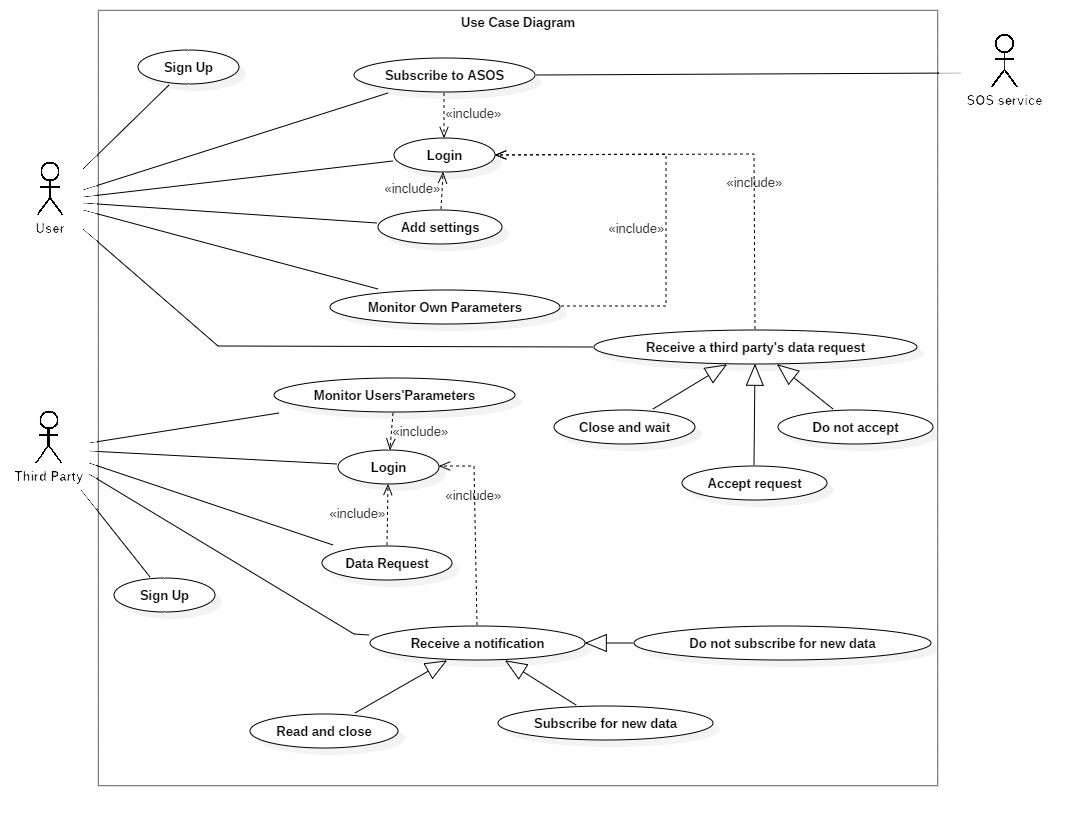
\includegraphics[width=1.1\textwidth]{./pictures/usecase_diagram.png}\par
	\caption{Figure 1: Use Case Diagram}
\end{figure}

\FloatBarrier

\subsubsection{Sign up}
\begin{center}
	\begin{longtable}{ | p{0.3\textwidth} | p{0.7\textwidth} | }
		\hline 
		 \A &  Sign Up \\ 

		\hline
		 \B &  User - Third party \\  %è da dividere?? sono necessari due diversi use cases??

		\hline
  		 \C &  The individual or the third party has downloaded the app on his/her smartphone.\\ 

		\hline
		 \D & \begin{enumerate}
			\item The individual opens the app on his/her smartphone;
			\item He/she clicks on the \textit{Register here} link;
			\item The user fills all the mandatory fields and provide all his/her personal data;
			\item He/she clicks on "Register" button;
			\item The system saves all personal data and creates a new personal area.
		\end{enumerate} \\

		\hline
		 \E &  The user has a personal area and now he/she is able to use the application.\\

		\hline
		 \F & \begin{enumerate}
			\item The user is already signed up
			\item The user didn’t fill all of the mandatory fields;
			\item The e-mail has already been registered;
			\item All the exceptions are handled by notifying the user and taking him back to the sign up activity.
		\end{enumerate} \\
		
		\hline
		 \G &  G1 - G2\\

		\hline
		 \H &  R1 - R3- R4 - R6 \\
		\hline

	\end{longtable}
\end{center}

\subsubsection{Login}
\begin{center}
	\begin{longtable}{ | p{0.3\textwidth} | p{0.7\textwidth} | }
		\hline
		 \A &   Login \\ 

		\hline
		 \B &  User - Third party \\ 

		\hline
  		 \C &  The user or the third party has the application installed; has succesfully registered and has a personal area.\\ 

		\hline
		\D & \begin{enumerate}
			\item The user  or the third party opens the app on his/her smartphone;
			\item Writes his/her credentials;
			\item Clicks on "Login" button;
		\end{enumerate} \\

		\hline
		\E & The user  or the third party is succesfully redirected to his/her main page.\\

		\hline
		\F & \begin{enumerate}
			\item The user or the third party doesn't register yet;
			\item The user or the third party enters an invalid Username;
			\item The user or the third party enters an invalid Password;
			\item He/she doesn't fill all fields.
		\end{enumerate} All the exceptions are handled by notifying the user and taking him/her back to the login activity. \\
		
		\hline
		\G & G1 - G2\\

		\hline
		\H & R2 - R3.1- R5 - R6.1 \\
		\hline

	\end{longtable}
\end{center}

\subsubsection{Add settings details}
\begin{center}
	\begin{longtable}{ | p{0.3\textwidth} | p{0.7\textwidth} | }
		\hline
		 \A &   Add settings details\\ 

		\hline
		 \B &  User \\ 

		\hline
  		 \C &  The user has the application installed; has successfully registered; has a personal area and has a device that can be linked to the smartphone.\\ 

		\hline
		\D & \begin{enumerate}
			\item The user opens the app on his/her smartphone;
			\item He/she login;
			\item Opens the Menu by the three points icon in the main scene;
			\item Clicks on the \textit{Settings} link;
			\item Inserts his/her weight and height;
			\item Adds his/her device;
			\item Clicks the \textit{Save} button.
		\end{enumerate} \\

		\hline
		\E & The app saves successfully all personal data and the device starts to send health parameters.\\

		\hline
		\F & \begin{enumerate}
			\item The user exits from the Settings area without saving, this exception is handled by notifying it to the user;
			\item The user doesn't link any personal device, this exception can't be handled but the user notices it because 					without a linked device the app can't run correctely.
		\end{enumerate} \\
		
		\hline
		\G & G1\\

		\hline
		\H & R3.1 - R3.3 \\
		\hline

	\end{longtable}
\end{center}

\subsubsection{Monitor own parameters}
\begin{center}
	\begin{longtable}{ | p{0.3\textwidth} | p{0.7\textwidth} | }
		\hline
		 \A &  Monitor his/her own parameters\\ 

		\hline
		 \B &  User \\ 

		\hline
  		 \C &    The user has the application installed; has succesfully registered; has a personal area, has added settings details and has a device linked to his/her smartphone.\\

		\hline
		\D & \begin{enumerate}
			\item The user login;
		\end{enumerate} \\

		\hline
		\E & The app opens the main scene in which the user can see his/her health paramters by graphs and numbers.\\

		\hline
		\F & - \\
		
		\hline
		\G & G7\\

		\hline
		\H & R20\\
		\hline

	\end{longtable}
\end{center}

\subsubsection{Receive a third party's data request}
In the figure 3.21 there are three use cases which derives from this abstract one; their difference is given by the last step of the event flow and the exit condition. Because of this reason we have chosen to compress them in just one table.
\begin{center}
	\begin{longtable}{ | p{0.3\textwidth} | p{0.7\textwidth} | }
		\hline
		 \A &   Receive a notification\\ 

		\hline
		 \B &  User \\ 

		\hline
  		 \C &  The user has the application installed; has succesfully registered; has a personal area and has a device linked to his/her smartphone.\\ 

		\hline
		\D & \begin{enumerate}
			\item The user receives a notification on his/her smartphone;
			\item He/she login and finds an alert;
			\item Reads the alert;
			\item Click on the \textit{Accept} button or on the \textit{Refuse} button or on the \textit{Exit} icon.
		\end{enumerate} \\

		\hline
		\E & The allert is closed and the choise is saved: \begin{enumerate}
			\item if he/she has clicked on the \textit{Exit} icon the notification is added in the \textit{Data Request Notification} 				area;
			\item if he/she has clicked on the \textit{Accept} button the third party is added in the \textit{Third Party} area;					\item else it is delated.
		\end{enumerate}\\

		\hline
		\F & \begin{enumerate}
			\item The user doesn't accept neither refuse before the time bound.
		\end{enumerate} This exception is resolved by considering the non answer as a negative one. \\
		
		\hline
		\G & G4\\

		\hline
		\H & R3.2 - R9 - R10 \\
		\hline

	\end{longtable}
\end{center}

\subsubsection{Receive a notification (third party)}
In the figure 3.21 there are three use cases which derives from this abstract one; their difference is given by the last step of the event flow and the exit condition. Because of this reason we have chosen to compress them in just one table.
\begin{center}
	\begin{longtable}{ | p{0.3\textwidth} | p{0.7\textwidth} | }
		\hline
		 \A &   Receive a notification\\ 

		\hline
		 \B &  Third Party \\ 

		\hline
  		 \C &  The third party has the application installed; has succesfully registered and has a personal area.\\ 

		\hline
		\D & \begin{enumerate}
			\item The third party receives a notification;
			\item The third party login and finds an alert;
			\item Reads the alert;
			\item Clicks on the \textit{Subscribe} button or on the \textit{Refuse} button or on the \textit{Exit} icon.
		\end{enumerate} \\

		\hline
		\E & The allert is closed and the choise is saved: \begin{enumerate}
			\item if the third party  has clicked on the \textit{Subscribe} button the single user data or the group of users data are 				added in the main scene and the third party will always receive new data ;					
			\item  if the third party  has clicked on the \textit{Refuse} button the single user data or the group of users data are 				added in the main scene and the third party won't receive new data ;	
			\item else nothing happens.
		\end{enumerate}\\

		\hline
		\F & -\\
		\hline
		\G & G5 - G6\\

		\hline
		\H & R6.1 - R11 - R12 - R13 - R14 - R15 - R16\\
		\hline

	\end{longtable}
\end{center}

\subsubsection{Subscribe to \textit{ASOS}}
\begin{center}
	\begin{longtable}{ | p{0.3\textwidth} | p{0.7\textwidth} | }
		\hline
		 \A &   Subscribe to \textit{ASOS}\\ 

		\hline
		 \B &  User \\ 

		\hline
  		 \C &  The user has the application installed; has succesfully registered; has a personal area and has a device linked to the smartphone.\\ 

		\hline
		\D & \begin{enumerate}
			\item He/she login;
			\item Opens the menu and clicks on the \textit{ASOS} link;
			\item Checks the check boxes;
			\item Clicks on the \textit{Save} button.
		\end{enumerate} \\

		\hline
		\E & The app saves the choise and activate the \textit{ASOS} service.\\

		\hline
		\F & - \\
		
		\hline
		\G & G7 - G8\\

		\hline
		\H & R17 - R18 - R19 \\
		\hline

	\end{longtable}
\end{center}

\subsubsection{Data request}
\begin{center}
	\begin{longtable}{ | p{0.3\textwidth} | p{0.7\textwidth} | }
		\hline
		 \A &  Request data\\ 

		\hline
		 \B &  Third Party \\ 

		\hline
  		 \C &  The third party has the application installed; has succesfully registered and has a personal area.\\

		\hline
		\D & \begin{enumerate}
			\item The third party login;
			\item Clicks on the plus icon in the main scene: if the request is for single user data the first one else the second;
			\item Fills all the mandatory fields with the required data  ;
			\item Clicks on the \textit{Save and Send request} button.
		\end{enumerate} \\

		\hline
		\E & The app saves the request and starts to elaborate it.\\

		\hline
		\F & \begin{enumerate}
			\item The third party doesn't fill any field.
		\end{enumerate} The exception is handled by notifying the third party and taking him back to the Request Data activity. \\
		
		\hline
		\G & G3 - G3.1 - G3.2\\

		\hline
		\H & R6.2 - R7 - R8 - R8.1 \\
		\hline

	\end{longtable}
\end{center}

\subsubsection{Monitor users' parameters}
\begin{center}
	\begin{longtable}{ | p{0.3\textwidth} | p{0.7\textwidth} | }
		\hline
		 \A &  Monitor users' parameters\\ 

		\hline
		 \B &  Third Party \\ 

		\hline
  		 \C &  The third party has the application installed; has succesfully registered; has a personal area and has received data of some single users and some group of users.\\

		\hline
		\D & \begin{enumerate}
			\item The third party login;
			\item Clicks on a \textit{Fiscal code X} button or on a \textit{Group X} button;
		\end{enumerate} \\

		\hline
		\E & The app opens the health parameter of the user associated to the clicked fiscal code or to the group of users associated to the considered group.\\

		\hline
		\F & - \\
		
		\hline
		\G & G6\\

		\hline
		\H & R6.1 - R15 \\
		\hline

	\end{longtable}
\end{center}
\subsection{Sequence Diagrams}
In this section are reported the most meaningful sequence diagrams in relation to some scenarios previously presented.

\begin{figure}[!h]
	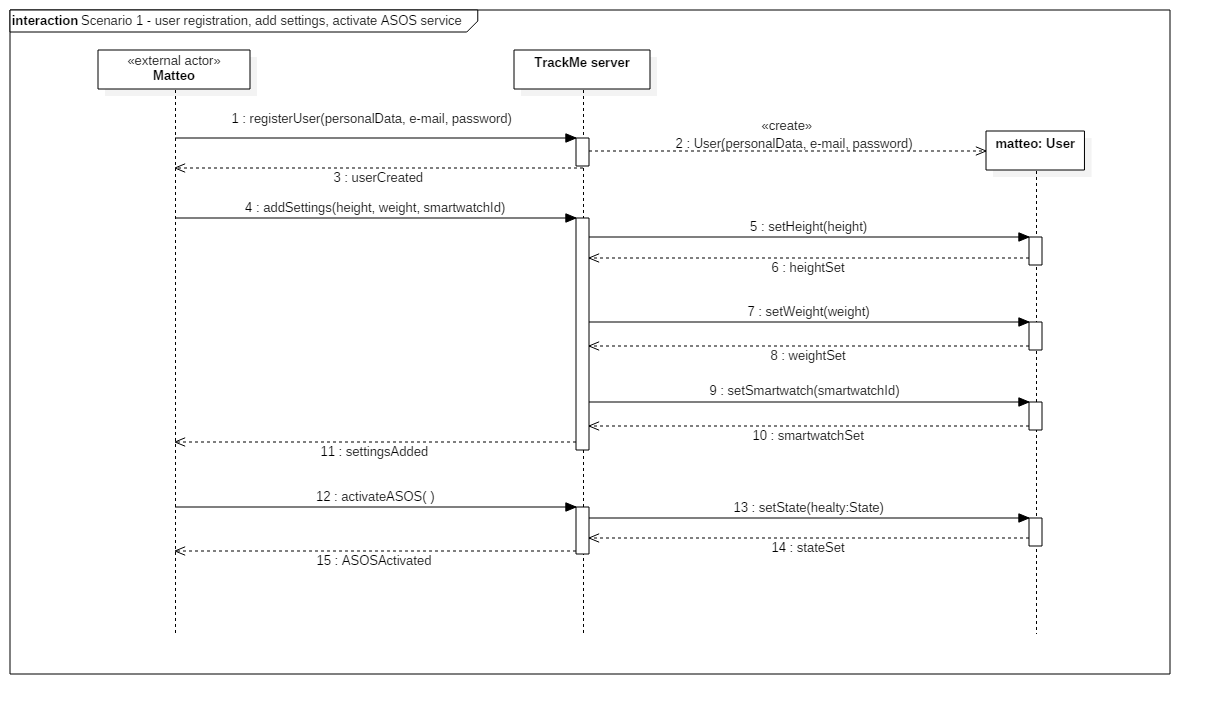
\includegraphics[width=1.00\textwidth]{./pictures/Scenario_1.png}\par
	\caption{Figure 1: Sequence diagram relative to the scenario 1.}
\end{figure}
\FloatBarrier
\vspace{0.3cm}

\begin{figure}[!h]
	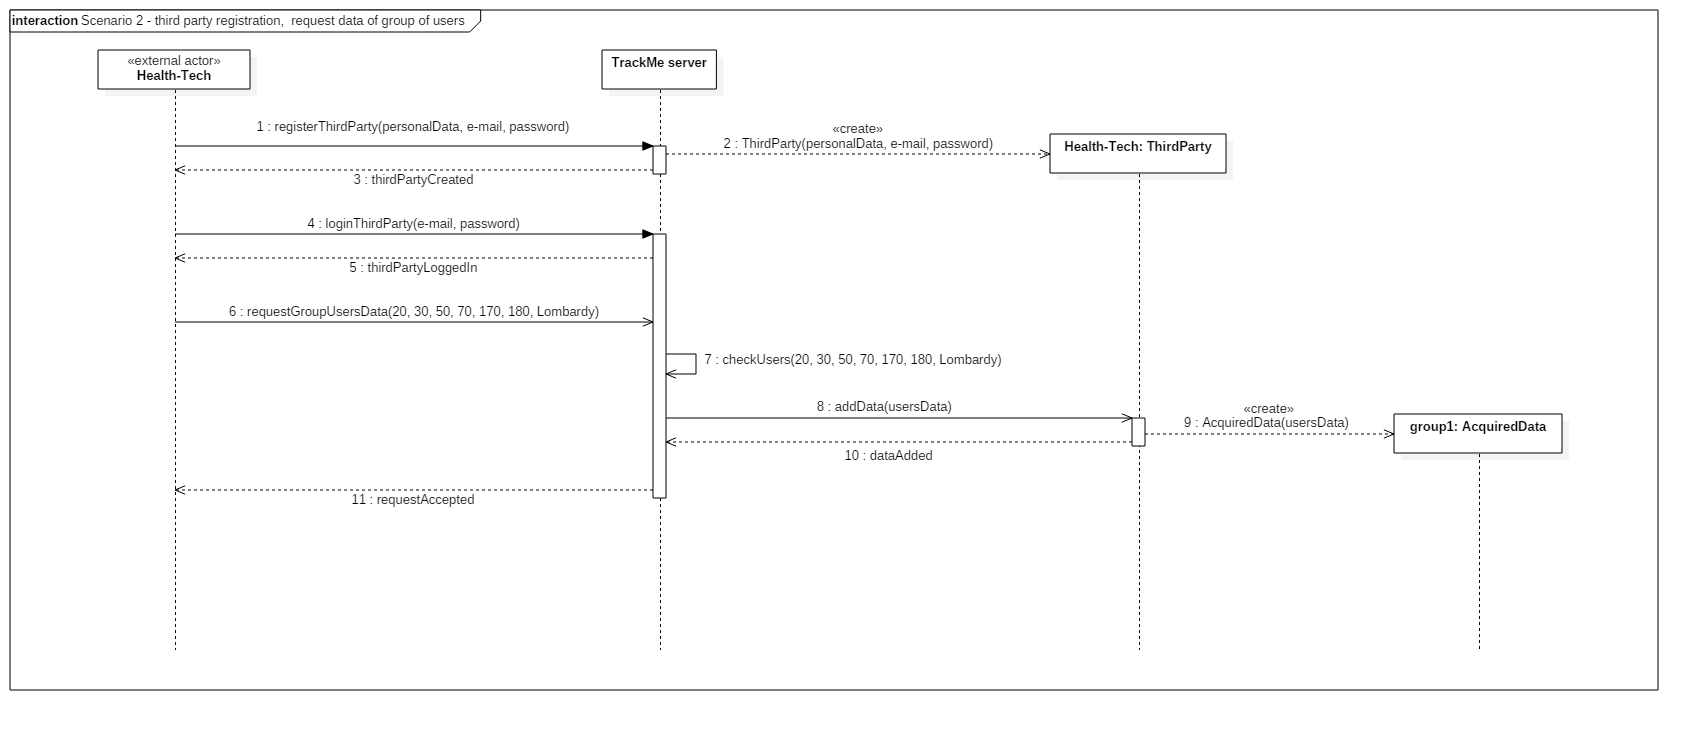
\includegraphics[width=1.00\textwidth]{./pictures/Scenario_2.png}\par
	\caption{Figure 2: Sequence diagram relative to the scenario 2.}
\end{figure}
\FloatBarrier
\vspace{0.3cm}

\begin{figure}[!h]
	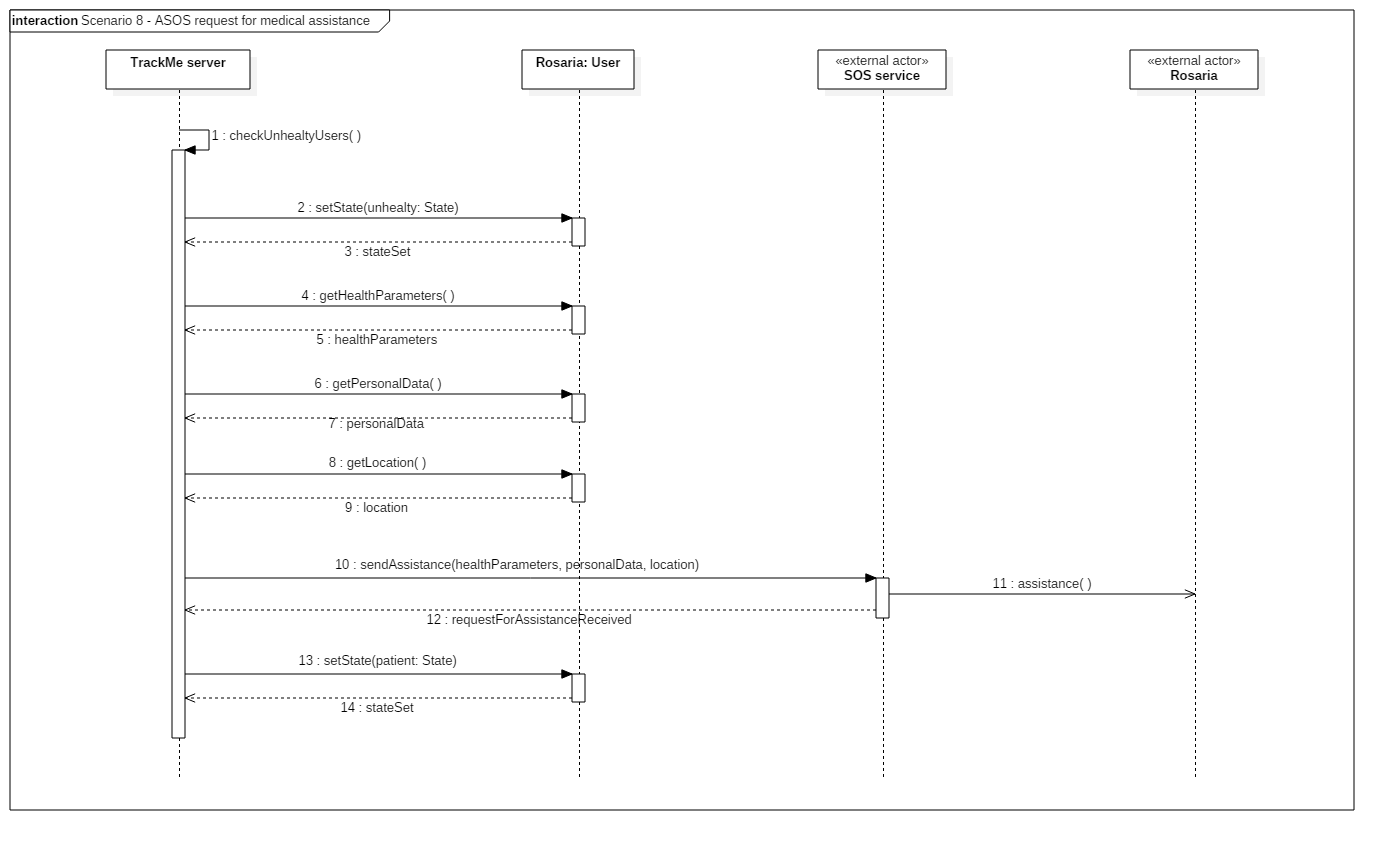
\includegraphics[width=1.00\textwidth]{./pictures/Scenario_8.png}\par
	\caption{Figure 3: Sequence diagram relative to the scenario 8.}
\end{figure}
\FloatBarrier
\vspace{0.3cm}


	\section{Performance Requirements} 
	The system is provided to serve fairly great number of users and third parties simultaneously.
%dobbiamo aggiungere dei numeri o restiamo molto generici??
Users will rely on the application in order to monitor their health parameters and to receive help in case of parameters lower than the threshold. Third party will rely on the application in order to require data of single user or group of users.

	\section{Design Constraints}
	\subsection{Standard compliance}
%still missing

\subsection{Hardware limitations}
The app for users requires a smartphone and a device that are compatible and which can be linked one to each other.\\
The smartphone must have the following properties:
\begin{itemize}
	\item GPS;
	\item bluetooth;
	\item 3G or 4G internet connection;
	\item Android or IOS system.

\end{itemize}The app for third parties requires a smartphone which has a 3G or 4G connection and an Android or IOS system.

\subsection{Regulatory policies}
The system must be allowed by users and third parties to collect, process and store their personal data; it also must be capable to delete them if a user or a third party requires it. While signing up users must give the permission to the system to share their data in an anonymized way and in the personal privacy respect.\\
Users and third parties must use the system in a propert way respecting law and policies.
	
	\section{Software System Attributes} 
	\subsection{Reliability}
The application must be available 24/7. Negligibly small concessions might be tolerated.

\subsection{Availability}
In order to guarantee high degree of availability, system of redundant servers may be considered. This way, if possibly one server fails, the other one will be ready to take over.  The system is expected to be available 99.99 percent of the time for the users which have subscibed to \textit{ASOS}.

\subsection{Security}
Users and third parties credential should be confidentially stored and encrypted with high-security encryption. It must be guarantee to users that their data will be anonymized if they will be shared with a third party which has required a group of users data.

\subsection{Maintainability}
The app is going to be flexible and easy to maintain, i.e capable to facilitate addition of new features and options. For that purpose we will use clear code following the design patterns as much as possible. \\
Complete and detailed documentation will be provided in order to keep Maintainabilityt on the highest level.

\subsection{Portability}


	%Alloy Model
	\chapter{Alloy} 
	\label{ch: alloy}

	%Appendix
	\appendix
	\chapter{Appendix}



\end{document}